\documentclass[aspectratio=169, 10pt]{beamer}

% ─────────────────────────────────────────────
%  THEME & COLOUR PALETTE (Clean White Theme)
% ─────────────────────────────────────────────
\usetheme{Madrid}
\usecolortheme{default}

\definecolor{acrNavy}{HTML}{0D1B2A}
\definecolor{acrSlate}{HTML}{1B3A5C}
\definecolor{acrBlue}{HTML}{2E6DA4}
\definecolor{acrIce}{HTML}{A8D8EA}
\definecolor{acrAccent}{HTML}{00C9A7}
\definecolor{acrGold}{HTML}{F5A623}
\definecolor{acrLight}{HTML}{EFF4FB}
\definecolor{acrRed}{HTML}{E84A5F}
\definecolor{acrGray}{HTML}{8492A6}

% Clean white backgrounds
\setbeamercolor{palette primary}{bg=acrBlue, fg=white}
\setbeamercolor{palette secondary}{bg=acrSlate, fg=white}
\setbeamercolor{palette tertiary}{bg=acrNavy, fg=white}
\setbeamercolor{structure}{fg=acrBlue}
\setbeamercolor{frametitle}{bg=acrNavy, fg=white}
\setbeamercolor{title}{fg=acrNavy}
\setbeamercolor{subtitle}{fg=acrBlue}
\setbeamercolor{background canvas}{bg=white}
\setbeamercolor{normal text}{fg=acrNavy}

\setbeamercolor{block title}{bg=acrBlue, fg=white}
\setbeamercolor{block body}{bg=acrLight, fg=acrNavy}
\setbeamercolor{block title alerted}{bg=acrRed, fg=white}
\setbeamercolor{block body alerted}{bg=acrLight!50!white, fg=acrNavy}
\setbeamercolor{block title example}{bg=acrAccent!80!black, fg=white}
\setbeamercolor{block body example}{bg=acrLight!50!white, fg=acrNavy}
\setbeamercolor{itemize item}{fg=acrAccent}
\setbeamercolor{itemize subitem}{fg=acrBlue}

% ─────────────────────────────────────────────
%  PACKAGES
% ─────────────────────────────────────────────
\usepackage[T1]{fontenc}
\usepackage[utf8]{inputenc}
\usepackage{graphicx}
\usepackage{xcolor}
\usepackage{booktabs}
\usepackage{tikz}
\usetikzlibrary{shapes.geometric,arrows.meta,positioning,shadows}
\usepackage{listings}
\usepackage{pifont}
\usepackage{tcolorbox}
\tcbuselibrary{skins,breakable}

% ─────────────────────────────────────────────
%  SYMBOL MACROS
% ─────────────────────────────────────────────
\newcommand{\symCheck}{\textcolor{acrAccent}{\ding{52}}}
\newcommand{\symWarn}{\textbf{\textcolor{acrRed}{[!]}}}
\newcommand{\symAST}{\textbf{\textcolor{acrAccent}{[AST]}}}
\newcommand{\symCode}{\textbf{\textcolor{acrAccent}{\{/\}}}}
\newcommand{\symDB}{\textbf{\textcolor{acrBlue}{[DB]}}}
\newcommand{\symCI}{\textbf{\textcolor{acrAccent}{[CI]}}}
\newcommand{\symBrain}{\textbf{\textcolor{acrAccent}{[AI]}}}

% ─────────────────────────────────────────────
%  LISTINGS
% ─────────────────────────────────────────────
\lstdefinestyle{shellstyle}{
  language=bash,
  basicstyle=\ttfamily\scriptsize\color{white},
  backgroundcolor=\color{acrNavy},
  keywordstyle=\color{acrAccent}\bfseries,
  stringstyle=\color{acrGold},
  commentstyle=\color{acrGray}\itshape,
  frame=single,
  rulecolor=\color{acrBlue},
  numbers=none,
  breaklines=true,
  showstringspaces=false,
  xleftmargin=4pt,
  xrightmargin=4pt,
}

\lstdefinestyle{yamlstyle}{
  basicstyle=\ttfamily\scriptsize\color{white},
  backgroundcolor=\color{acrNavy},
  keywordstyle=\color{acrAccent}\bfseries,
  stringstyle=\color{acrGold},
  commentstyle=\color{acrGray}\itshape,
  frame=single,
  rulecolor=\color{acrBlue},
  numbers=none,
  breaklines=true,
  showstringspaces=false,
  xleftmargin=4pt,
  xrightmargin=4pt,
}

% ─────────────────────────────────────────────
%  BEAMER SETUP
% ─────────────────────────────────────────────
\setbeamerfont{frametitle}{size=\large,series=\bfseries}
\setbeamerfont{title}{size=\huge,series=\bfseries}
\setbeamertemplate{itemize item}{\textcolor{acrAccent}{\ding{118}}}
\setbeamertemplate{itemize subitem}{\textcolor{acrBlue}{\ding{111}}}
\setbeamertemplate{navigation symbols}{}

% ─────────────────────────────────────────────
%  META
% ─────────────────────────────────────────────
\title[ACR-QA v2.7]{ACR-QA Phase 2 Progress Update}
\subtitle{Competitive Features \& Production Readiness}
\author{Ahmed Mahmoud Abbas}
\institute[KSIU]{King Salman International University\\Supervisor: Dr.\ Samy Abdelnabi}
\date{March 11, 2026}

% ═════════════════════════════════════════════
%  DOCUMENT
% ═════════════════════════════════════════════
\begin{document}

% ─── SLIDE 1 — TITLE ─────────────────────────
\begin{frame}[plain]
  \vspace{1.0cm}
  \centering
  \IfFileExists{media/ksiu-logo.png}{
\includegraphics[height=1.5cm]{media/ksiu-logo.png}\\[0.5em]}{}
  {\Huge\bfseries\color{acrNavy} ACR-QA}\\[0.3em]
  {\Large\color{acrBlue} Phase 2 Progress Update}\\[0.5em]

  \begin{tcolorbox}[
    enhanced,colback=acrLight,colframe=acrAccent,
    coltext=acrNavy,width=0.8\linewidth,center,
    boxrule=1pt,arc=5pt
  ]
    \centering\small
    \textbf{Enterprise Features} \quad\textbullet\quad
    \textbf{Rigorous Testing} \quad\textbullet\quad
    \textbf{Production CI/CD}
  \end{tcolorbox}

  \vspace{0.5cm}
  {\small\color{acrSlate} \textbf{Ahmed Mahmoud Abbas} \quad\textbullet\quad King Salman International University}\\[0.2em]
  {\small\color{acrSlate} \textbf{Supervisor: Dr.\ Samy Abdelnabi} \quad\textbullet\quad \today}\\[0.5em]
\end{frame}

% ─── SLIDE 2 — CONTEXT REFRESHER ─────────────
\begin{frame}{Quick Refresher: What is ACR-QA?}
  \begin{columns}[T]
    \begin{column}{0.65\textwidth}
      \textbf{A multi-tool, RAG-enhanced code quality platform.}
      \vspace{0.5em}
      \begin{itemize}\setlength\itemsep{0.6em}
        \item Explains \textit{why} code is problematic and \textit{how} to fix it.
        \item Uses Groq AI + RAG (Retrieval-Augmented Generation).
        \item Consolidates 7 static analysis engines.
        \item Zero recurring cost (open-source engines).
      \end{itemize}
    \end{column}
    \begin{column}{0.35\textwidth}
      \begin{tcolorbox}[colback=acrLight,colframe=acrBlue,title=\textbf{Core Stack}]
        \scriptsize \symCode{} FastAPI\\ \symDB{} PostgreSQL/Redis\\ \symBrain{} Groq AI\\ \symCI{} GitHub Actions
      \end{tcolorbox}
    \end{column}
  \end{columns}
\end{frame}

% ─── SLIDE 3 — THE MASSIVE LEAP ──────────────
\begin{frame}{From Prototype to Enterprise (Jan 18 $\rightarrow$ Today)}
  \begin{columns}[T]
    \begin{column}{0.48\textwidth}
      \begin{tcolorbox}[colback=acrLight,colframe=acrSlate,title={\textbf{Jan 18\textsuperscript{th} (v2.0)}}]
        \small
        \begin{itemize}
          \item Working prototype
          \item Basic detection + AI
          \item $\sim$30 basic tests
        \end{itemize}
      \end{tcolorbox}
    \end{column}
    \begin{column}{0.48\textwidth}
      \begin{tcolorbox}[colback=white,colframe=acrAccent,title={\textbf{Today (v2.7)}}]
        \small
        \begin{itemize}
          \item Enterprise CI/CD product
          \item Policy-as-Code engine
          \item \textbf{273 rigorous tests}
        \end{itemize}
      \end{tcolorbox}
    \end{column}
  \end{columns}
  \vspace{1em}
  \textbf{Key Pillars Added:}
  \begin{itemize}
    \item \textbf{Reliability:} 273 tests, simulated DB failures, 100\% pass rate.
    \item \textbf{DevOps:} GitHub Actions, Prometheus metrics.
    \item \textbf{Innovation:} Competitive features absent in paid tools (SonarQube).
  \end{itemize}
\end{frame}

% ─── SLIDE 4 — ENTERPRISE ARCHITECTURE ───────
\begin{frame}[fragile]{Enterprise Architecture \& Policy-as-Code}
    \begin{columns}[T]
    \begin{column}{0.55\textwidth}
      \begin{itemize}\setlength\itemsep{1em}
        \item \textbf{Quality Gates (Policy-as-Code)}
          \begin{itemize}
            \item Define pass/fail rules in \texttt{.acrqa.yml}.
            \item Pipeline predictably blocks bad code.
          \end{itemize}
        \item \textbf{Inline Suppression}
          \begin{itemize}
            \item Ignore specific lines via \texttt{\# acr-qa:ignore}.
          \end{itemize}
        \item \textbf{Language Adapters}
          \begin{itemize}
            \item Core restructured. JS/TS support easily pluggable.
          \end{itemize}
      \end{itemize}
    \end{column}
    \begin{column}{0.45\textwidth}
      \begin{tcolorbox}[colback=acrNavy,title={\textbf{.acrqa.yml Example}},coltext=white]
\begin{lstlisting}[style=yamlstyle]
quality_gates:
  critical_issues: 0
  high_issues: 5
  test_coverage: 80

suppression:
  enabled: true
  keyword: "acr-qa:ignore"
\end{lstlisting}
      \end{tcolorbox}
    \end{column}
  \end{columns}
\end{frame}

% ─── SLIDE 5 — INNOVATION I ──────────────────
\begin{frame}[fragile]{Innovation I: The Test Gap Analyzer}
  \begin{columns}[T]
    \begin{column}{0.6\textwidth}
      \textbf{The Problem:}
      Coverage metrics (80\%) hide \textit{which} critical logic is untested.

      \vspace{1em}
      \textbf{Our Solution:}
      \begin{itemize}\setlength\itemsep{0.5em}
        \item Custom \textbf{AST parser} scans logic.
        \item Identifies exact untested functions.
        \item Ranks them by \textbf{cyclomatic complexity} (not line count).
        \item Fails CI/CD if complex business logic is skipped.
      \end{itemize}
    \end{column}
    \begin{column}{0.4\textwidth}
      \begin{tcolorbox}[colback=acrNavy,title={\textbf{CI/CD Output}},coltext=white]
\begin{lstlisting}[style=shellstyle]
UNTESTED CRITICAL:
 process_payment()
  complexity: 24
 validate_token()
  complexity: 18

[FAIL] Pipeline blocked
\end{lstlisting}
      \end{tcolorbox}
    \end{column}
  \end{columns}
\end{frame}

% ─── SLIDE 6 — INNOVATION II ─────────────────
\begin{frame}[fragile]{Innovation II: Security \& Compliance}
  \begin{columns}[T]
    \begin{column}{0.55\textwidth}
      \begin{itemize}\setlength\itemsep{1em}
        \item \textbf{OWASP Top 10 Mapping}
          \begin{itemize}
            \item Every finding automatically mapped to OWASP categories and CWE IDs.
          \end{itemize}
        \item \textbf{Automated Compliance Reports}
          \begin{itemize}
            \item Generates audit-ready reports on every pipeline run.
          \end{itemize}
        \item \textbf{Policy Engine Validator}
          \begin{itemize}
            \item Validates \texttt{.acrqa.yml} strictly, preventing silent pipeline failures.
          \end{itemize}
      \end{itemize}
    \end{column}
    \begin{column}{0.45\textwidth}
      \begin{tcolorbox}[colback=acrNavy,title={\textbf{Security Output}},coltext=white]
\begin{lstlisting}[style=shellstyle]
[CRITICAL] SQL Injection
 Rule: B608
 OWASP: A03:2021
 CWE-ID: CWE-89

 Fix: Use parameters.
 AI: "String interpolation
 allows attackers..."
\end{lstlisting}
      \end{tcolorbox}
    \end{column}
  \end{columns}
\end{frame}

% ─── SLIDE 7 — INNOVATION III ────────────────
\begin{frame}[fragile]{Innovation III: Developer Fatigue Tuner}
  \begin{columns}[T]
    \begin{column}{0.55\textwidth}
      \textbf{The Problem:}
      Developers abandon tools due to false positive spam.

      \vspace{1em}
      \textbf{Our Solution (Feedback Tuner):}
      \begin{itemize}\setlength\itemsep{0.5em}
        \item Learns from dashboard `false positive' votes.
        \item Calculates FP rates continuously.
        \item \textbf{Auto-dials down severity} of noisy rules.
        \item Suppresses AI explanations if confidence $< 0.70$.
      \end{itemize}
    \end{column}
    \begin{column}{0.45\textwidth}
      \begin{tcolorbox}[colback=acrNavy,title={\textbf{Live Adaptation}},coltext=white]
\begin{lstlisting}[style=shellstyle]
[TUNER] Rule: E501
 FP Rate: 73%
 Action: HIGH -> INFO
 Reason: High FP rate.

[TUNER] AI filtered:
 conf=0.61 < 0.70
\end{lstlisting}
      \end{tcolorbox}
    \end{column}
  \end{columns}
\end{frame}

% ─── SLIDE 8 — RELIABILITY ───────────────────
\begin{frame}{Comprehensive Reliability (v2.7)}
  \begin{columns}[T]
    \begin{column}{0.6\textwidth}
      \begin{itemize}\setlength\itemsep{1em}
        \item \textbf{Rigorous Test Architecture}
          \begin{itemize}
            \item Scaled to \textbf{273 tests} (unit, integration, stress).
          \end{itemize}
        \item \textbf{High Performance}
          \begin{itemize}
            \item Full 273-test suite executes in $< 6$ seconds.
          \end{itemize}
        \item \textbf{Stress Tested}
          \begin{itemize}
            \item Simulated corrupt DBs, 1,000-finding streams, missing files (Zero crashes).
          \end{itemize}
        \item \textbf{100\% CI/CD Pass Rate} on GitHub.
      \end{itemize}
    \end{column}
    \begin{column}{0.4\textwidth}
      \centering
      \vspace{0.5em}
      {\fontsize{40}{45}\selectfont\bfseries\color{acrAccent} 273}\\
      {\large\color{acrSlate} Passing Tests}\\[1em]

      {\fontsize{28}{32}\selectfont\bfseries\color{acrGold} $<$ 6s}\\
      {\large\color{acrSlate} Execution Time}\\[1em]
    \end{column}
  \end{columns}
\end{frame}

% ─── SLIDE 9 — GITHUB PROFESSIONALIZATION ────
\begin{frame}{Ready for the Real World}
  \begin{columns}[T]
    \begin{column}{0.5\textwidth}
      \begin{itemize}\setlength\itemsep{1em}
        \item \textbf{Live PR Inline Comments}
          \begin{itemize}
            \item Auto-posts inline code review comments on GitHub Pull Requests.
          \end{itemize}
        \item \textbf{Official Releases}
          \begin{itemize}
            \item v2.7.0 published with semantic versioning and changelogs.
          \end{itemize}
        \item \textbf{Tracked Roadmap}
          \begin{itemize}
            \item Phase 2 fully scoped via organized GitHub Issues.
          \end{itemize}
      \end{itemize}
    \end{column}
    \begin{column}{0.5\textwidth}
      \IfFileExists{media/pr-comment-mockup1.png}{
        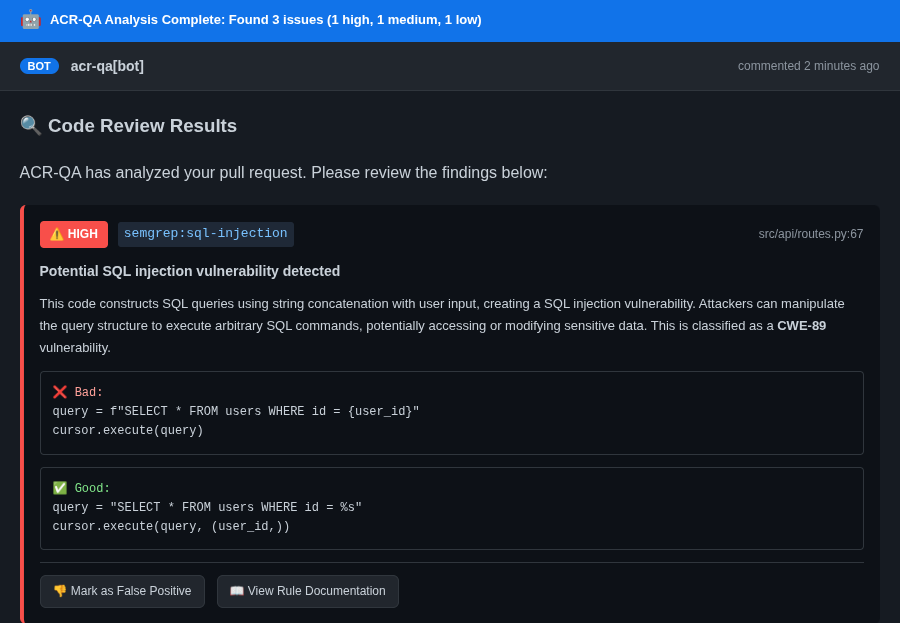
\includegraphics[width=\textwidth,keepaspectratio]{media/pr-comment-mockup1.png}
      }{
        \vspace{1cm}
        \centering\textit{(Live PR integration active on repo)}
      }
    \end{column}
  \end{columns}
\end{frame}

% ─── SLIDE 10 — NEXT STEPS ───────────────────
\begin{frame}{Roadmap: Phase 2 Launch}
  \begin{columns}[T]
    \begin{column}{0.32\textwidth}
      \begin{tcolorbox}[colback=acrLight,colframe=acrAccent,title={\textbf{Language Expansion}}, height=5cm]
        \small
        \begin{itemize}
          \item Launching JS/TS parsing.
          \item Adapter pattern is ready.
        \end{itemize}
      \end{tcolorbox}
    \end{column}
    \begin{column}{0.32\textwidth}
      \begin{tcolorbox}[colback=acrLight,colframe=acrGold,title={\textbf{Scientific Validation}}, height=5cm]
        \small
        \begin{itemize}
          \item User studies with developers.
          \item Precision / Recall benchmark tests.
        \end{itemize}
      \end{tcolorbox}
    \end{column}
    \begin{column}{0.32\textwidth}
      \begin{tcolorbox}[colback=acrLight,colframe=acrBlue,title={\textbf{Cloud Readiness}}, height=5cm]
        \small
        \begin{itemize}
          \item AWS / GCP deployment.
          \item Live demo for final defense.
        \end{itemize}
      \end{tcolorbox}
    \end{column}
  \end{columns}
\end{frame}

\end{document}
